\documentclass{llncs}
\usepackage[utf8]{inputenc}
\usepackage[OT4]{fontenc}
\usepackage{hyperref}
\usepackage{amsmath,amssymb}
\usepackage{stmaryrd}
\usepackage{graphicx}

\newcommand{\pc}{\ensuremath\mathcal{K}}
\newcommand{\soi}{\ensuremath\mathcal{L}}
\newcommand{\next}{\ensuremath\mathcal{N}}
\newcommand{\ont}{\ensuremath\mathcal{O}}
\newcommand{\tbox}{\ensuremath\mathcal{T}}
\newcommand{\abox}{\ensuremath\mathcal{A}}
\newcommand{\soc}{\ensuremath\underline{\pc}}
\DeclareMathOperator{\POD}{pod}
\newcommand{\comment}[1]{\emph{#1}}

\title{Technical report: integration of inductive learning with formal concept analysis for ontology refinement}
\author{Jędrzej Potoniec}
\institute{Poznan University of Technology}
\begin{document}
\maketitle
\begin{abstract}
\end{abstract}

\section{Formal concept analysis}

Following description of formal concept analysis is based on \cite{baader2007completing}.

Let $M$ be a set of attributes. \emph{Partial object description (pod)} is a
tuple $(A,S)$ such that $A,S\subseteq M$. If $A\cup S=M$, this tuple is
\emph{full object description}. Set of pods is called \emph{partial context}
and set of fods is called \emph{full context}.

\emph{Implications} considered in formal concept analysys are of form
$L\rightarrow R$, where $L,R\subseteq M$. Implication is \emph{refuted by pod}
$(A,S)$ iff $A\subseteq L \land S\cap R\neq\emptyset$. Implication is
\emph{refuted by partial context} if it is refuted by at least one pod from
this partial context.

\begin{definition}
Let $\pc$ be a partial context and let $P\subseteq M$. 
$\pc(P)$ defined as follows is the largest subset of $M$ such that implication $P\to \pc(P)$ is not refuted by $\pc$.
\[ \pc(P)=M\backslash \bigcup_{\substack{(A,S)\in\pc\\P\subseteq A}} S \]
\end{definition}

\begin{definition}
Let $\soi$ be a set of implications. $\soi(P)\subseteq M$ is \emph{implicational closure} of set of attributes $P\subseteq M$ iff:
\begin{itemize}
\item $P\subseteq\soi(P)$
\item If $L\to R\in\soi$ and $L\subseteq \soi(P)$, then $R\subseteq\soi(P)$.
\item $\soi(P)$ is smallest set holding both above conditions.
\end{itemize}
If $\soi(P)=P$, then $P$ is called $\soi$-closed.
\end{definition}
0
\begin{definition}
Let $M=\{m_1,m_2,\ldots,m_n\}$ such that attributes are ordered ascendingly w.r.t. some linear order on $M$. For any two sets $P,Q\subseteq M$ and for any $i=1,2,\ldots,n$
\[P<_i Q \equiv \left(m_i\in Q\backslash P \land P\cap \{m_1,\ldots,m_{i-1}\}=Q\cap \{m_1,\ldots,m_{i-1}\} \right) \]

\emph{Lectic order $<$} is union of orders $<_i$: $<=<_1 \cup <_2 \cup \ldots \cup <_n$.
\end{definition}

\begin{definition}
Let $f(P,i)=\soi((P\cap \{m_1,\ldots,m_{i-1}\})\cup\{m_i\})$ for every $\soi$-closed $P\subseteq M$ and every $i=1,2,\ldots,n$.
$\next(P)$ is next $\soi$-closed set following $P$ w.r.t. the lettic order $<$: 
\[\next(P)=f(P,j) \qquad j=\max\{i: P<_i f(P,i)\} \]
\end{definition}

Let $\ont=(\tbox,\abox)$ be some DL-ontology. Let $M$ be set of attributes expressed in DL. 
$\POD_\ont(a,M)$ is partial object description induced by an individual $a\in\abox$:
\[ \POD_\ont(a,M)=\left(\{C\in M: \ont\models C(a)\}, \{C\in M: \ont\models \lnot C(a)\}\right) \]
$\pc_{\ont,M}$ is partial context induced by the ontology w.r.t. set of attributes $M$
\[ \pc_{\ont,M}=\{\POD_\ont(a,M): a\in\abox \} \]

\begin{definition}[Algorithm of attribute exploration for DL KBs]
Input: $\ont, M$. Output: altered $\ont$.
\begin{enumerate}
\item $\soi\leftarrow \emptyset, P\leftarrow \emptyset$
\item\label{algdl:while} If $P=M$, then stop. \comment{All attributes have been considered.}
\item \comment{Considering implication $P\to\pc_{\ont,M}(P)$.}
\item If $P=\pc_{\ont,M}(P)$, then go to \ref{algdl:next}. \comment{Implication is trivial, because premises and conclusions are the same.}
\item If $\ont\models \bigsqcap P \sqsubseteq \bigsqcap \pc_{\ont,M}(P)$, then go to \ref{algdl:store}. \comment{Implication follows from $\ont$.}
\item Ask expert if implication is correct. If it is, go to \ref{algdl:store}.
\item Request expert to extend $\abox$ such that implication is refuted, but all implications in $\soi$ stay currect. Go to \ref{algdl:while}.
\item \label{algdl:store} $\soi\leftarrow \soi\cup \{P\to\pc_{\ont,M}(P)\backslash P\}$ \comment{Remember implication as correct.}
%\item $P\leftarrow \soi(P)$ \comment{Close $P$, as $\next(\cdot)$ is defined only for $\soi$-closed sets. This is not present in \cite{baader2007completing} and aparently for a reason, because it is not correct.}
\item \label{algdl:next} $P\leftarrow \next(P)$ \comment{Go to the next set of premises.}
\item Go to \ref{algdl:while}.
\end{enumerate}
\end{definition}

\begin{example}
\[ \tbox=\{Pociag, Szynobus, EZT, Pies, Szynobus\sqsubseteq Pociag \} \]
\begin{align*}
\abox=\{EZT(en57), Pociag(ed250), EZT(ed250), \lnot Szynobus(ed250),\\ Pociag(sa106), Pies(burek), Pies(reksiu) \}
\end{align*}
\[ M=\{Pociag, Szynobus, EZT, Pies\} \]
\end{example}

\section{Attribute exploration with special subset}

We consider users interested in extending knowledge base w.r.t. some set of
attributes $N\subseteq M$. It is not enough for them to set $M\leftarrow N$, as
this would stop them from finding implications with attributes from
$M\backslash N$.

\begin{definition}[interesting implication]
Implication $L\to R$ is \emph{interesting w.r.t. set $N$ of attributes} if $L\cap N\neq\emptyset \lor R\subseteq N$. In other words, implication is interesting if one of the following happens:
\begin{itemize}
\item premises contains at least one interesting attribute;
\item conclusions consists of only interesting attributes.
\end{itemize}
\end{definition}

\begin{definition}[set of interesting conclusions]
Let $P$ be premises of considered implication, $N$ set of interesting attributes and $\pc$ partial context. Set of interesting conclusions $\soc(P,N)$ is a set such that for every implication $L\to R\in\soc(P,N)$:
\begin{itemize}
\item this implication is interesting;
\item is no more general than implication $P\to\pc(P)$, i.e. $L\subseteq P \land R\subseteq \pc(P)$.
\end{itemize}
\[ \soc(P,N)=\begin{cases}
\{\pc(P)\} & P\cap N\neq\emptyset \\
\{\pc(P)\cap\pc(\{x\})\cap N : x\in N \} & \text{otherwise}
\end{cases} \]

In second part considered are only attributes which at the same time:
\begin{description}
\item[$\pc(P)$] are non-refuted by $P$;
\item[$\pc(\{x\})$] are non-refuted by at least one interesting attribute; \marginpar{but why?}
\item[$X$] are interesting.
\end{description}
\end{definition}

\begin{definition}[set of user-friendly interesting conclusions]
$\soc'(P,N)$ is a set of proper conclusions for $P$ which are single-attribute. This way users can decide more easily if implication is correct and automatic generation of counter-examples is easier.
\[ \soc'(P,N)=\{ \{x\} : \exists A\in\soc(P,N)\colon x\in A \} \]
\end{definition}

%Because $A\subseteq B \implies \pc(B)\subseteq\pc(A)$, so $\pc({x})$ is the biggest subset of attributes 

\begin{definition}[User-friendly algorithm of attribute exploration for DL KBs]
\ldots \marginpar{Find a clever way to describe iteration over $\soc'(P,N)$.}
\end{definition}


\section{Preparing partial context}

\begin{definition}[Linked Data mapping]
Let \emph{Linked Data mapping} be a tuple $(E,V,M)$, where:
\begin{description}
\item[$E$] is an identifier (address) of query answering service;
\item[$V$] is distincted variable in queries;
\item[$M$] is a set of actual mappings in form $A\leftarrow Q$, where $A\in M$ and $Q$ is a query pattern;
\end{description}
\end{definition}

\begin{example}[Learning about Middle-earth from DBpedia]
Consider the following mapping:
\begin{description}
\item[$E$] \url{http://dbpedia.org/sparql}
\item[$V$] \texttt{?x}
\item[$M$] ~\\ \begin{tabular}{p{.25\textwidth}p{.75\textwidth}}
Attribute & Pattern \\
\hline
Man & \texttt{?x dbp-prop:characterRace dbpedia:Man\_\%28Middle-earth\%29} \\
Noldor & \texttt{?x dbp-prop:characterCulture dbpedia:Noldor} \\
Spider-Demon & \texttt{?x dcterms:subject dbpedia:Category\%3AFictional\_demons, dbpedia:Category\%3AFictional\_spiders, dbpedia:Category\%3AMiddle-earth\_characters}
\end{tabular}
\end{description}

To enable attribute exploration with ontologies where $\abox=\emptyset$, the
following algorithm is used. $\abox$ obtained this way is not meant to be used
only as a seed for attribute exploration, not as part of final ontology. This
algorithm should provide witness for every mapped attribute that in fact this
attribute (more precisely: DL-concept related with this attribute) is
satisfiable.  
\begin{definition}[Algorithm for population of $\abox$]
\marginpar{Extend to multiple mappings.}
Input: mapping $(E,V,M)$. Output: $\abox$.

For every $A\leftarrow Q\in M$:
\begin{enumerate}
\item Obtain witness of attribute $A$, by posing to the service $E$ query equivalent to the following SPARQL query template:
\texttt{SELECT $V$ WHERE \{ $Q$ \} LIMIT 1}. Use obtained name $a$ as name of an individual in $\abox$: 
\[ \abox \leftarrow \abox \cup \{ A(a) \} \]
\item For every $A'\leftarrow Q'\in M$ such that $A\neq A'$ pose to the service $E$ query equivalent to the following SPARQL query template:
\texttt{ASK WHERE \{ $Q'$ \} BINDINGS $V$ \{($a$)\}}. If the answer is positive, alter $\abox$:
\[ \abox \leftarrow \abox \cup \{ A'(a) \} \] Otherwise ignore result, as it
is meaningless: it may mean that remote knowledge base is incomplete (and in
fact $A'(a)$), that knowledge base is complete but holds close-world assumption
(and in fact $\lnot A'(a)$) or that it is unknown if $A'(a)$ or $\lnot A'(a)$.
\end{enumerate}
\end{definition}

If mappings and/or remote knowledge base are errorneus, context obtained from
this $\abox$ requires manual correction, because otherwise attribute
exploration algorithm will be conformant with the principle \emph{garbage in,
garbage out}.

\end{example}

\section{Integrating machine learning algorithms into attribute exploration}

Algorithm of attribute exploration requires good amout of work from users in answering if implications are correct or wrong. One can observe that many of considered implications are of similar structure. It would be desirable if an algorithm would be able to learn from user decisions and gradually help him/her during the process answering more and more questions. Of course, it may happen that answer given by the algorithm is wrong. In this case it is far better to reject correct implication (as user just does not earn additional knowledge) than to accept a wrong one (because it creates cost for the user, as it requires manual detection and correction).

In classic approach for attribute exploration in DL KBs this would be hard to achieve, because of lack of counterexamples for rejected implications. If only implications with single attribute in conclusion are considered, counterexamples can be generated automatically. Moreover, it does not alter the properties of knowledge base as there is open-world assumption and no unique names assumption. For implication $P\to\{r\}$, new name $a$ is generated and $\abox$ is altered with the following expressions:
\begin{itemize}
\item $p(a)$ for every $p\in P$;
\item $\lnot r(a)$.
\end{itemize}

Task of deciding if implication is correct or wrong is represented as ternary classification task. Every implication is classified to one of the following classes:
\begin{description}
\item[correct] implication is remembered as correct and next implication is generated;
\item[wrong] new counterexample is generated, as described above;
\item[undecided] user is asked if implication is correct or wrong. 
\end{description}

\subsection{Implication features}

To use implication in classification task it must be transformed into feature vector. \ldots\ldots

\subsection{ML algorithms}

\ldots\ldots multilayer perceptrons are the best \ldots\ldots

\section{Implementation}

Java, handcrafted FCA library and Weka. OntoComP would require too much changing.

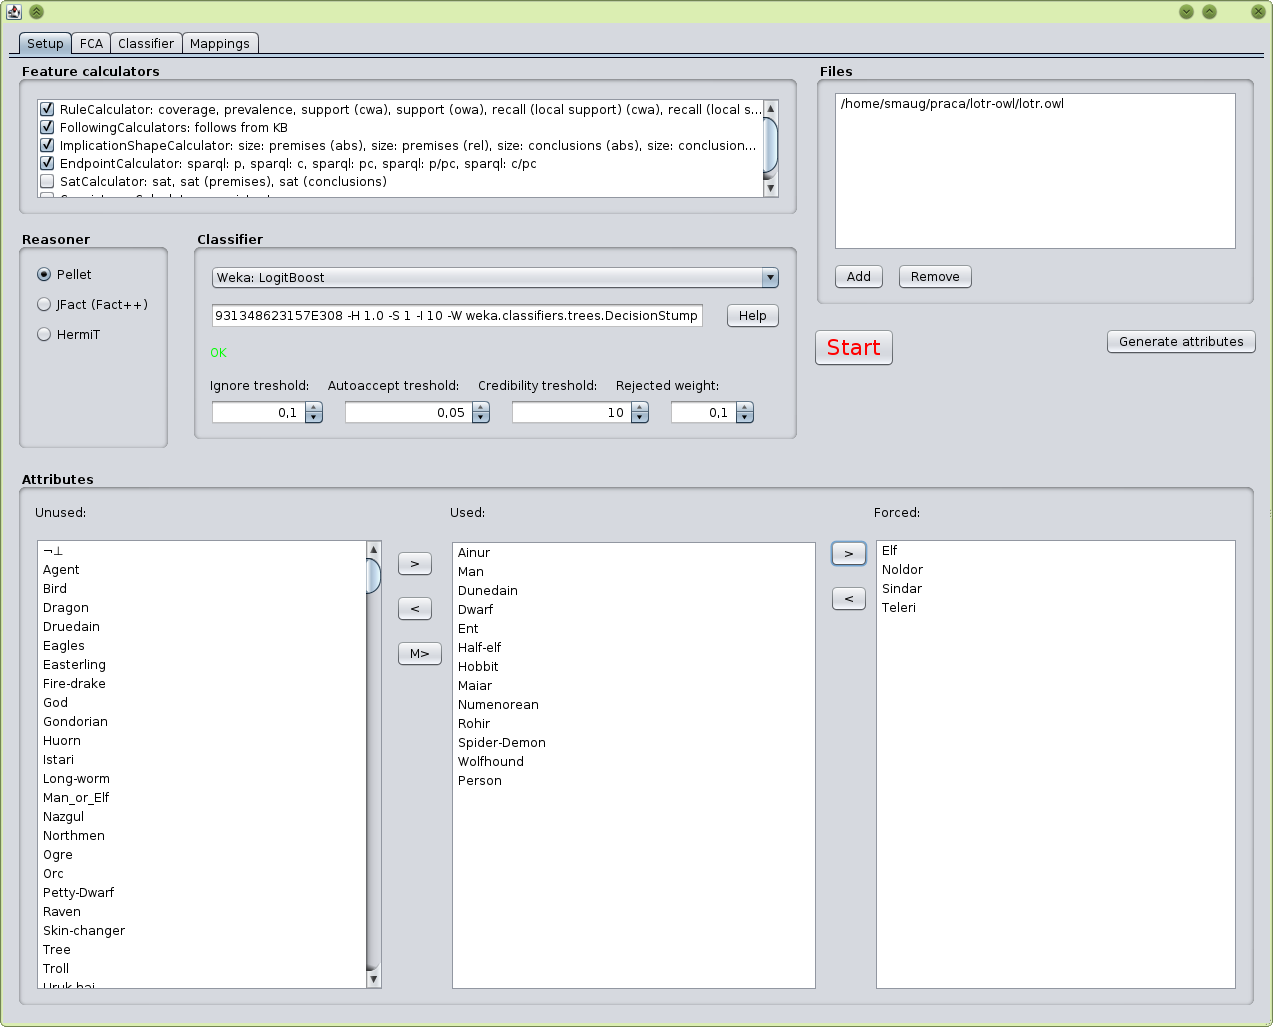
\includegraphics[width=\textwidth]{screenshots/setup.png}

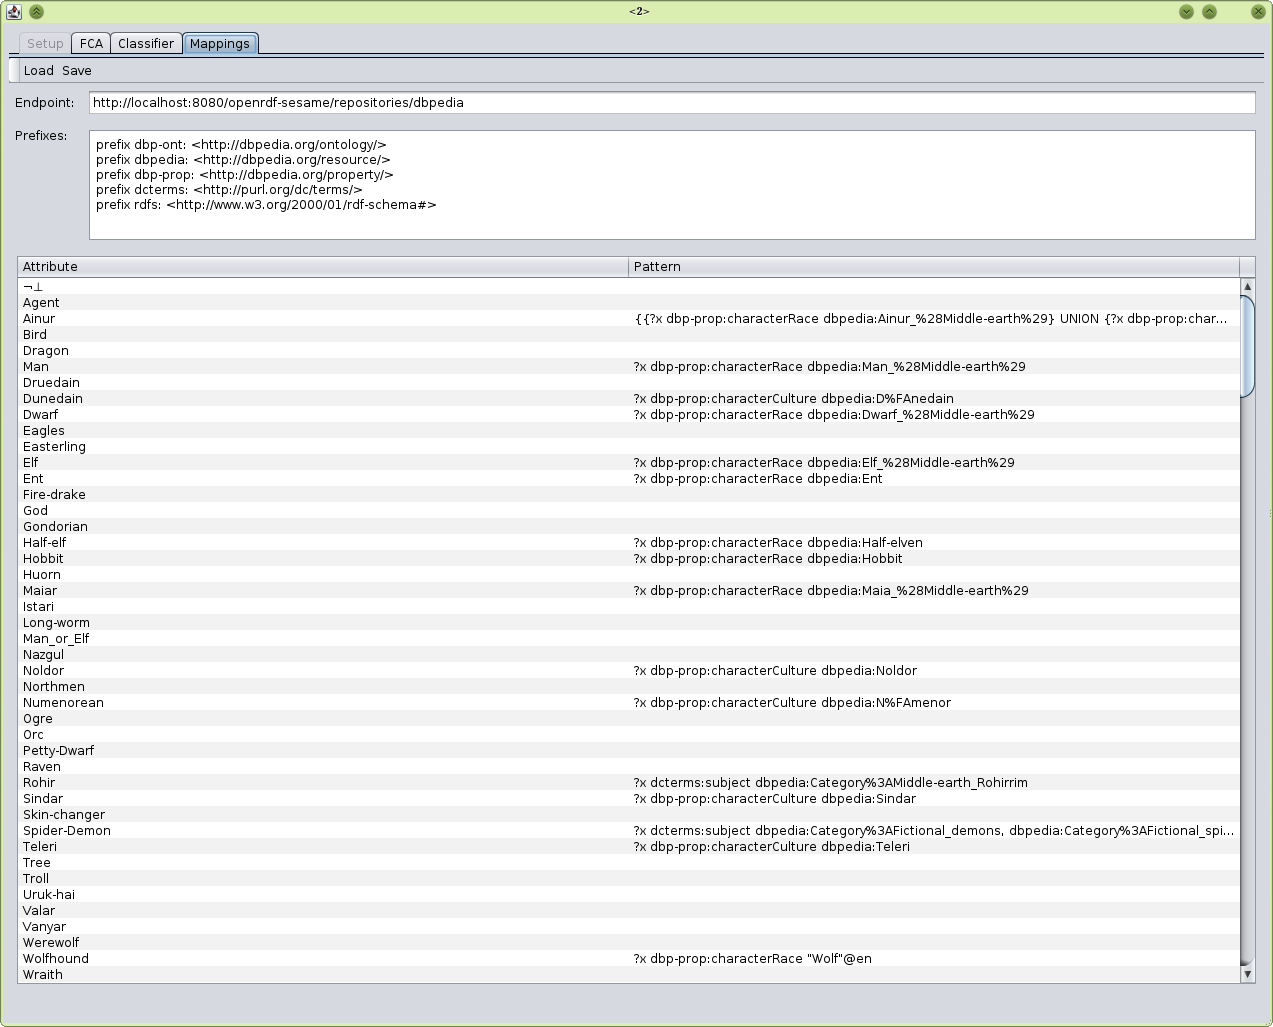
\includegraphics[width=\textwidth]{screenshots/mappings.png}

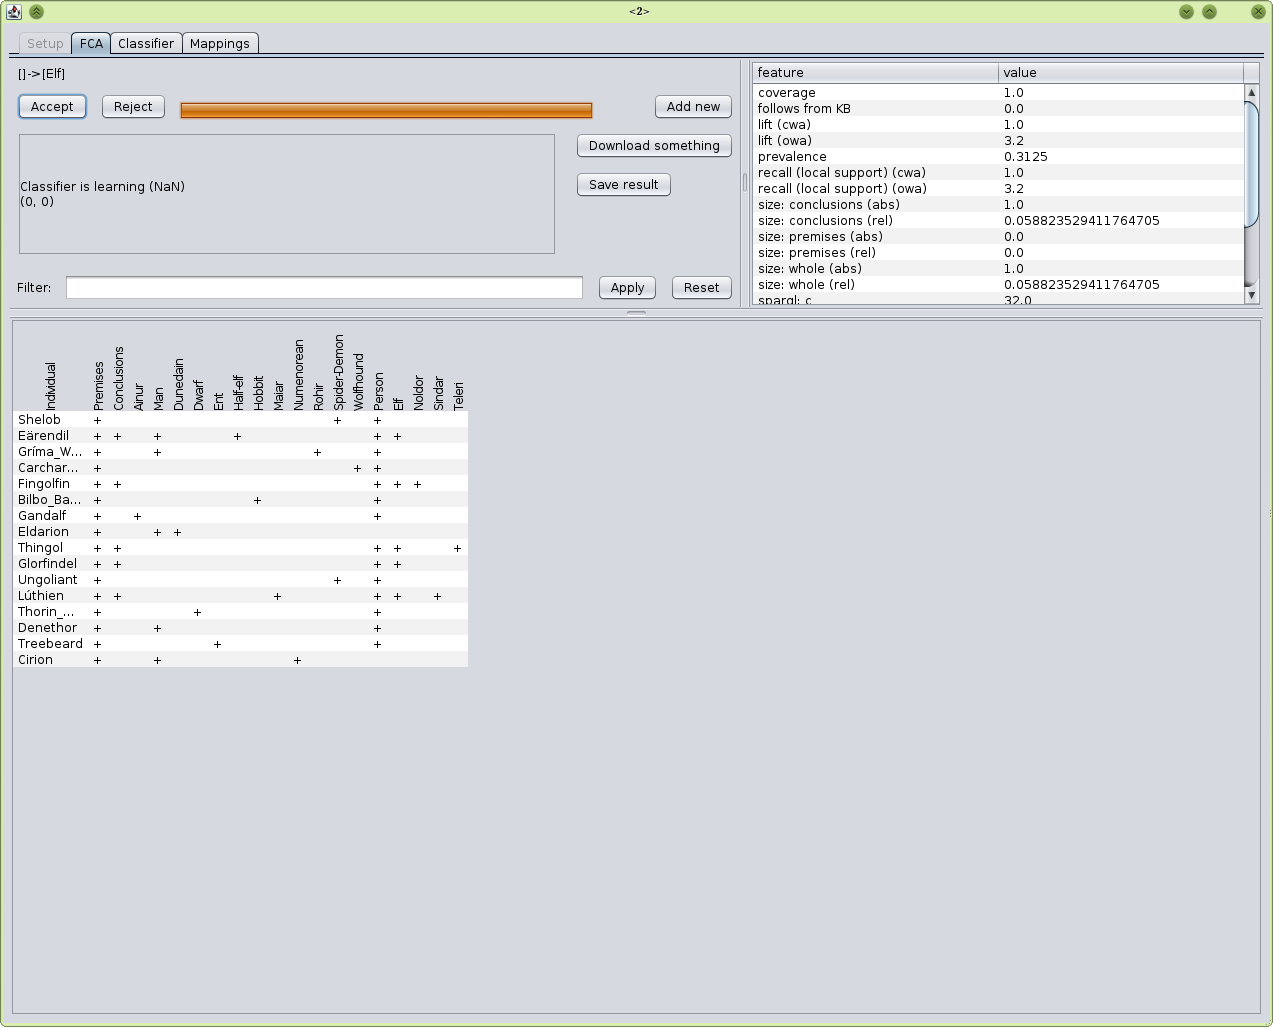
\includegraphics[width=\textwidth]{screenshots/fca1.png}

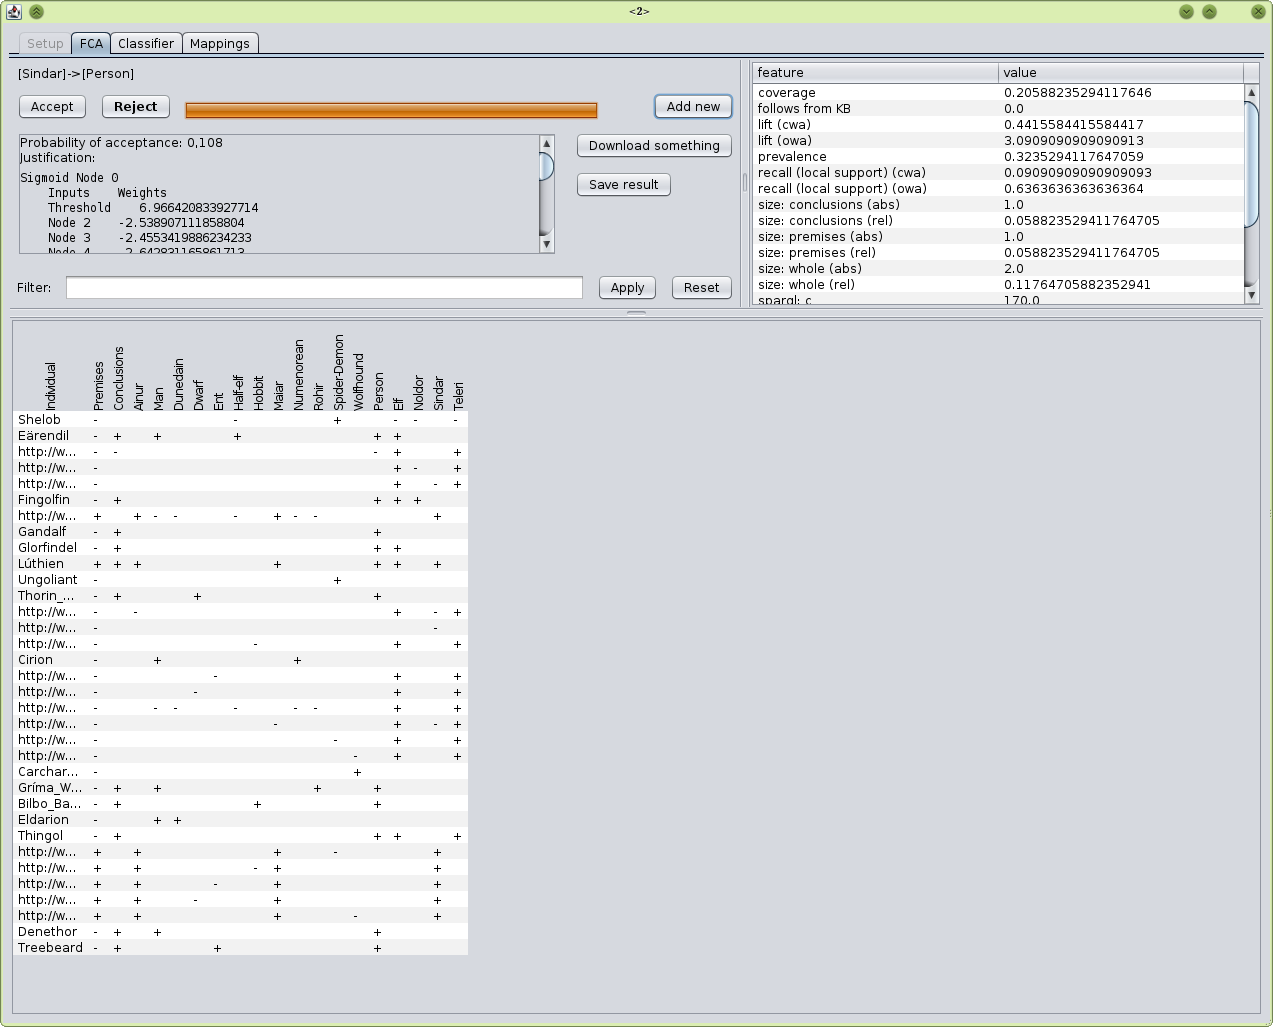
\includegraphics[width=\textwidth]{screenshots/fca2.png}

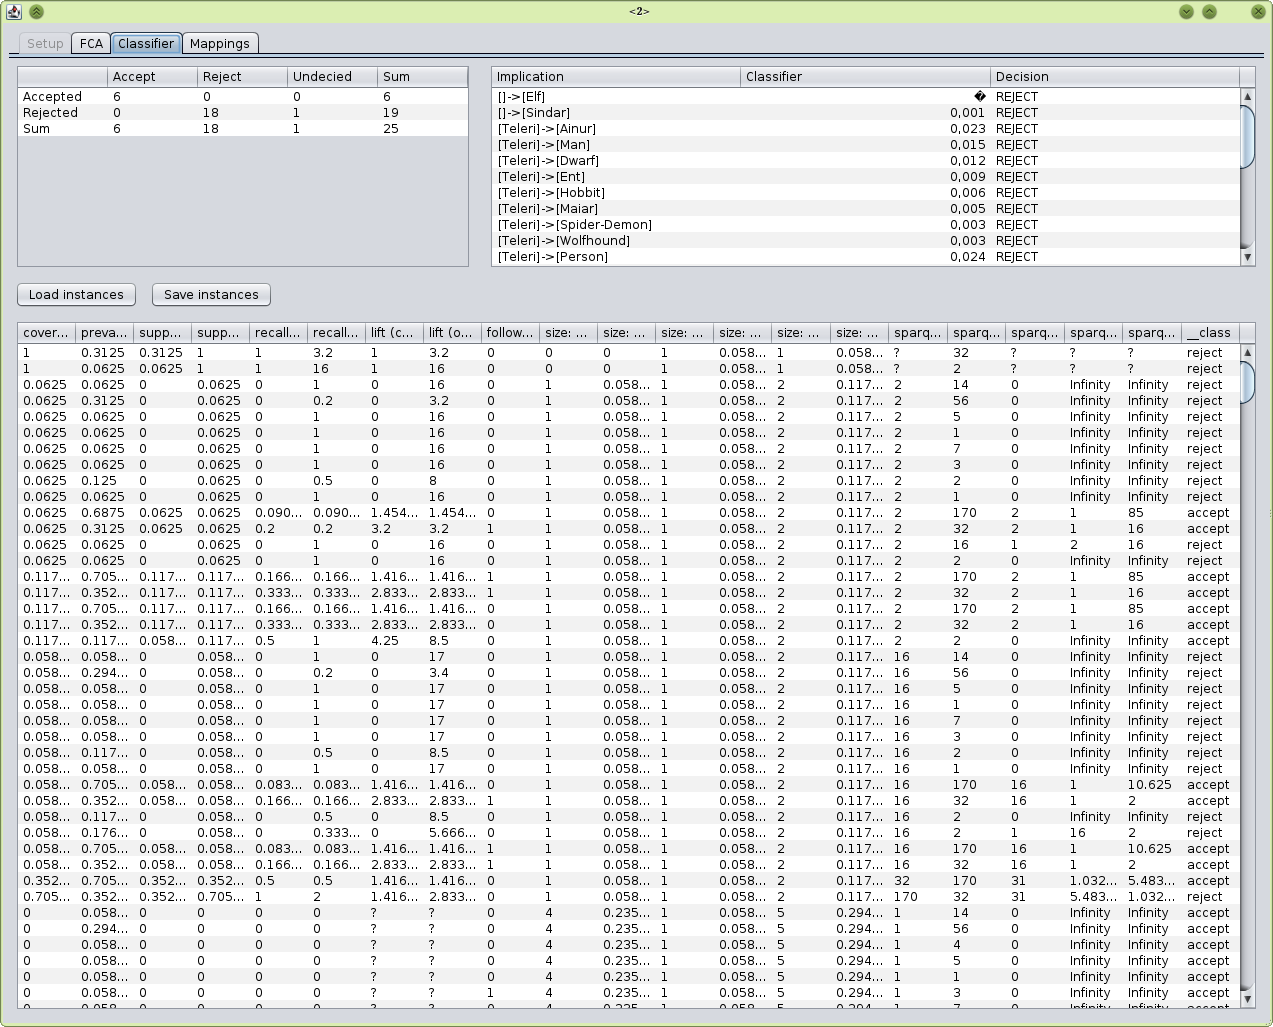
\includegraphics[width=\textwidth]{screenshots/classifier.png}

\bibliographystyle{plain}
\bibliography{report}

\end{document}
